\chapter{Projektumsetzung}
\label{cha:Projektumsetzung}

In diesem Kapitel wird die Implementierung des SCADA-Agenten anhand des im letzten Kapitel aufgezeigten Konzeptes erläutert.

\section{Übersetzten des Google V8 C++ Quellcodes}

Dieser Abschnitt beschreibt wie die Google V8 Quellcode in eine statische Bibliothek übersetzt werden kann.

\subsection{Linux}

Aufgrund der Compilervorgaben von WinCC OA gestaltet sich die Übersetzung des Quellcodes auf Linux schwierig. 
Das Google V8 Buildsystem ist auf Debian-Basierende Distributionen ausgelegt, das bedeutet die Engine kann auf dem Zielsystem
SUSE Linux Enterprise 12.5 nicht übersetzt werden. Ein alternativsystem mit der passenden Compilerversion stellt Ubuntu 18.04
zur Verfügung.

\begin{program}[h]
\caption{Installation von GCC-4.8.5 auf Ubuntu 18.04}
\label{src:inst_gcc}
\begin{GenericCode}
$ sudo apt update
$ sudo apt upgrade
$ sudo apt install git libglib2.0-dev python g++-4.8 gcc-4.8
$ sudo update-alternatives --install /usr/bin/gcc gcc /usr/bin/gcc-4.8 10
$ sudo update-alternatives --install /usr/bin/g++ g++ /usr/bin/g++-4.8 10
\end{GenericCode}
\end{program}

In dem Beispiel \ref{src:inst_gcc} ist gezeigt wie man auf einem Ubutu 18.04 System den benötigten Compiler nachinstallieren und als
Standardoption zum Übersetzten von Quellcode konfigurieren kann. Hat man diese Schritte durchgeführt, kann man die Google V8-Engine mit dem in Anhang 
\ref{app:v8build} gezeigten Skript kompilieren. Dabei werden zuerst automatisch der Quellcode und alle benötigten Dateien aus dem Google-Versionskontrollsystem 
bezogen. Als Nächstes wird eine Buildkonfiguration erzeugt. In dieser wird das Buildsystem angewiesen eine statische
Bibliothek zu generieren. Danach erfolgt eine Nachbearbeitung der generierten Dateien, weil die Standardkonfiguration einen neueren Compiler
voraussetzt. Hierbei wird die \textit{-std=gnu++14} Anweisung durch \textit{-std=gnu++11} ersetzt. Letztendlich wird der Buildprozess 
gestartet. Die fertigen Kompilate sind unter \textit{v8} und die Headerdateien unter \textit{include} zu finden und können auf einem SUSE Linux Enterprise 12.5
System verwendet werden. 

\subsection{Windows}

Auf Windows gestaltet sich dieser Prozess deutlich einfacher. Hier ist es zunächst nötig, Visual Studio 2015 zu installiert. Dadurch wird das \textit{Visual Studio Toolset} v140
zur Verfügung gestellt. Im nächsten Schritt muss man das in \ref{app:v8build} gezeigte Powershell-Skript für Windows mit folgendem Kommandozeilenparameter ausführen: 

\begin{GenericCode}[numbers=none]
$ powershell.exe -noprofile -executionpolicy bypass -file .\build_windows.ps1
\end{GenericCode}

Dadurch wird ähnlich wie unter Linux der Quellcode und weitere Dateien aus dem Google-Versionskontrollsystem bezogen, die Konfigurationsdateien erzeugt
und der Kompilevorgang angestoßen. Die übersetzten Bibliotheksdateien und die dazugehörigen Headerdateien befinden sich danach unter \textit{v8} und \textit{include}.

\section{Implementierung der Programmbibliothek}

Nun, da erklärt wurde, wie man ein Kompilat der Google V8 Engine als statische Bibliothek erhält, kann die auf die Implementierung der 
Programmkomponente eingegangen werden. Hierbei werden die einzelnen Klassen anhand deren UML-Repräsentation (\textit{Unified Modeling Language}) 
beschrieben. Das gesamte UML-Diagramm mit allen Relationen kann in Anhang \ref{app:classdiag} eingesehen werden.

\subsection{Implementierung der Singleton Klasse}

\begin{figure}[h]
	\centering 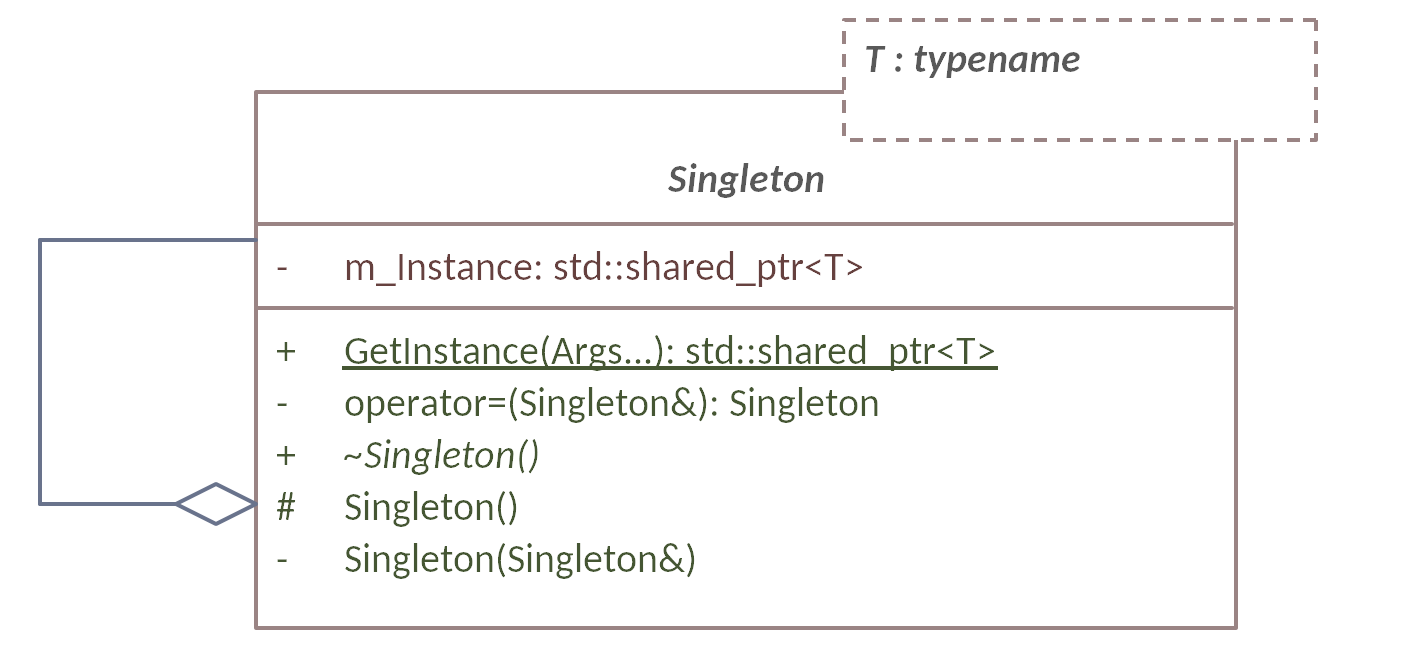
\includegraphics[width=0.63\textwidth]{singleton}
	\caption{Singleton Template-Klasse.}
	\label{fig:singleton}
\end{figure}

Diese in \ref{fig:singleton} gezeigte Template-Klasse implementiert eine wiederverwendbare Umsetzung des Singleton-Entwurfsmusters \cite{Singleton}. Ableitende Klassen erhalten indem sie
sich selbst als Template-Parameter übergeben eine \textit{GetInstance()} Funktion, die die einzige Instanz als \textit{Shared-Pointer} zurückgibt. 
Dadurch ist ein korrektes Freigeben des Speichers am Ende der Programmausführung gewährleistet. Ableitende Klassen müssen zusätzlich deren 
Konstruktor als \textit{protected} deklarieren und die Singleton klasse als \textit{friend} hinzufügen. Die \textit{GetInstance()} Methode nimmt
jene Parameter entgegen, die eine ableitende Klasse zur Konstruktion benötigt.

\subsection{Implementierung der libV8 Klasse}

\begin{figure}[h]
	\centering 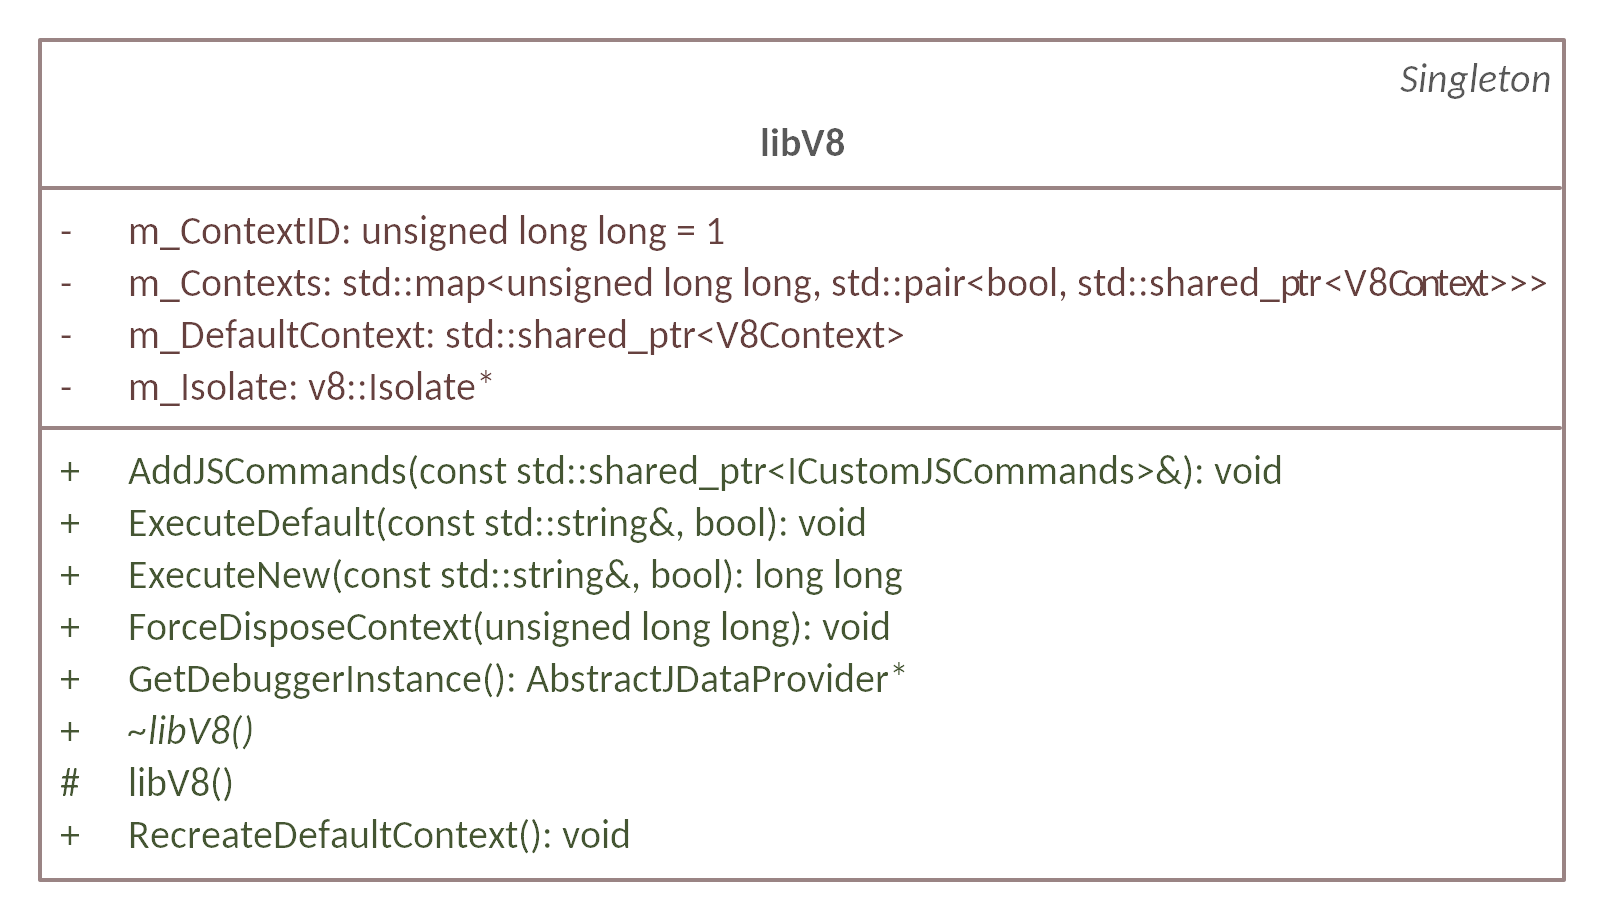
\includegraphics[width=0.63\textwidth]{libv8}
	\caption{Klassendiagramm der imlementierten Programmkomponente.}
	\label{fig:libv8}
\end{figure}

Abbildung \ref{fig:libv8} zeigt die Hauptkomponente der Bibliothek. Diese Klasse verwaltet das \textit{Isolate} Objekt der Google V8-Engine und alle
Ausführungsumgebungen. Über die Funktionen \textit{ExecuteDefault()} und \textit{ExecuteNew} ist es möglich Javascript-Dateien auszuführen. Beide akzeptieren
als ersten Parameter einen Pfad zu einer Skriptdatei und als zweiten einen booleschen wert der Angibt ob der Ausführungskontext am Ende des Skriptes zerstört 
werden soll oder nicht. 

\subsection{Implementierung der V8Context Klasse}


\begin{figure}[h]
	\centering 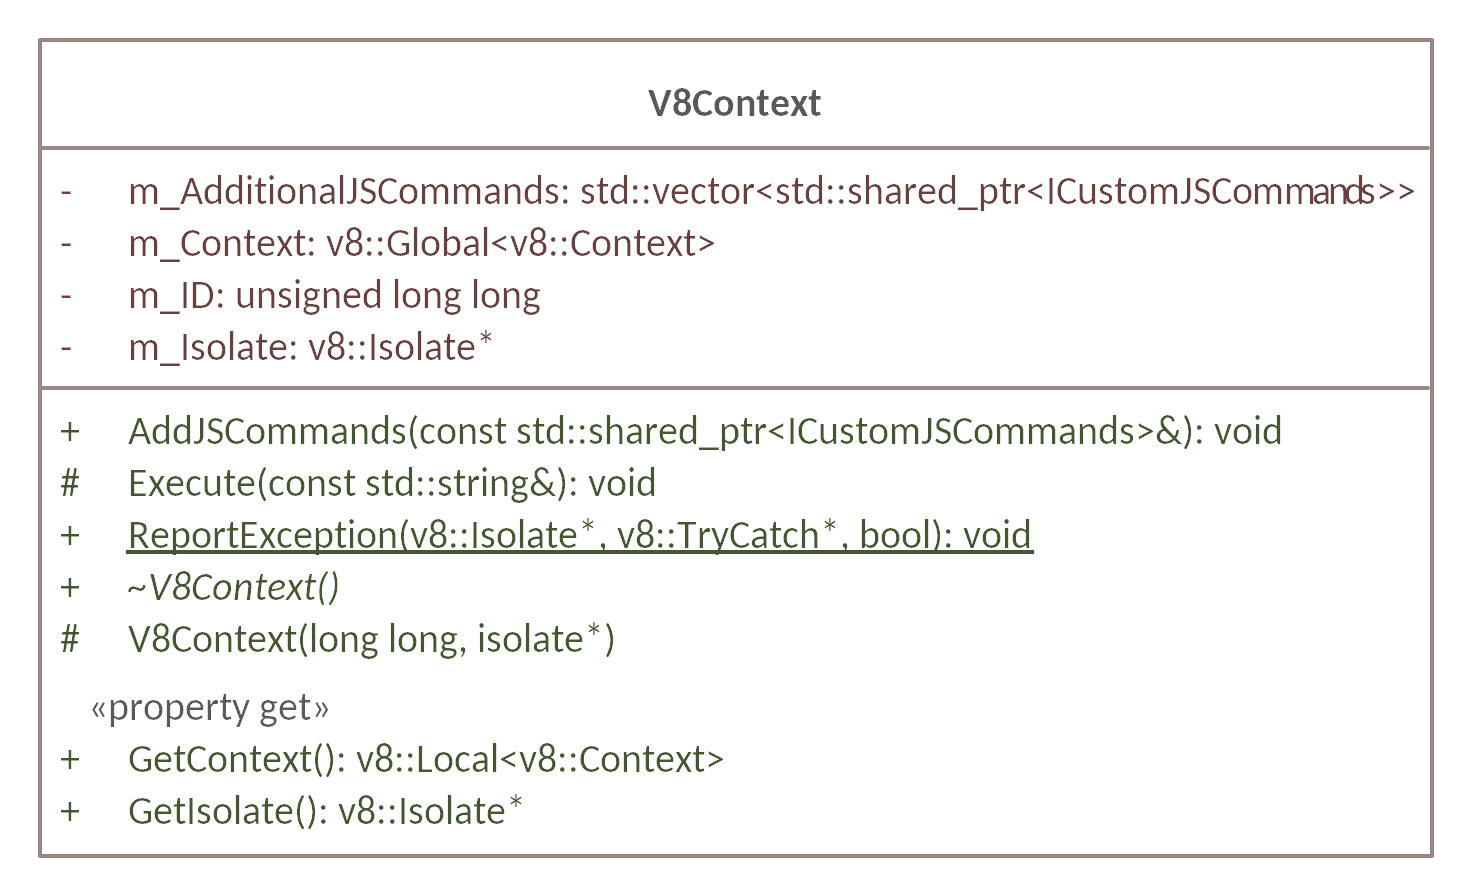
\includegraphics[width=0.63\textwidth]{v8context}
	\caption{Klassendiagramm der imlementierten Programmkomponente.}
	\label{fig:classdiag}
\end{figure}


\subsection{Implementierung der SIS\_InspectorClient Klasse}

\begin{figure}[h]
	\centering 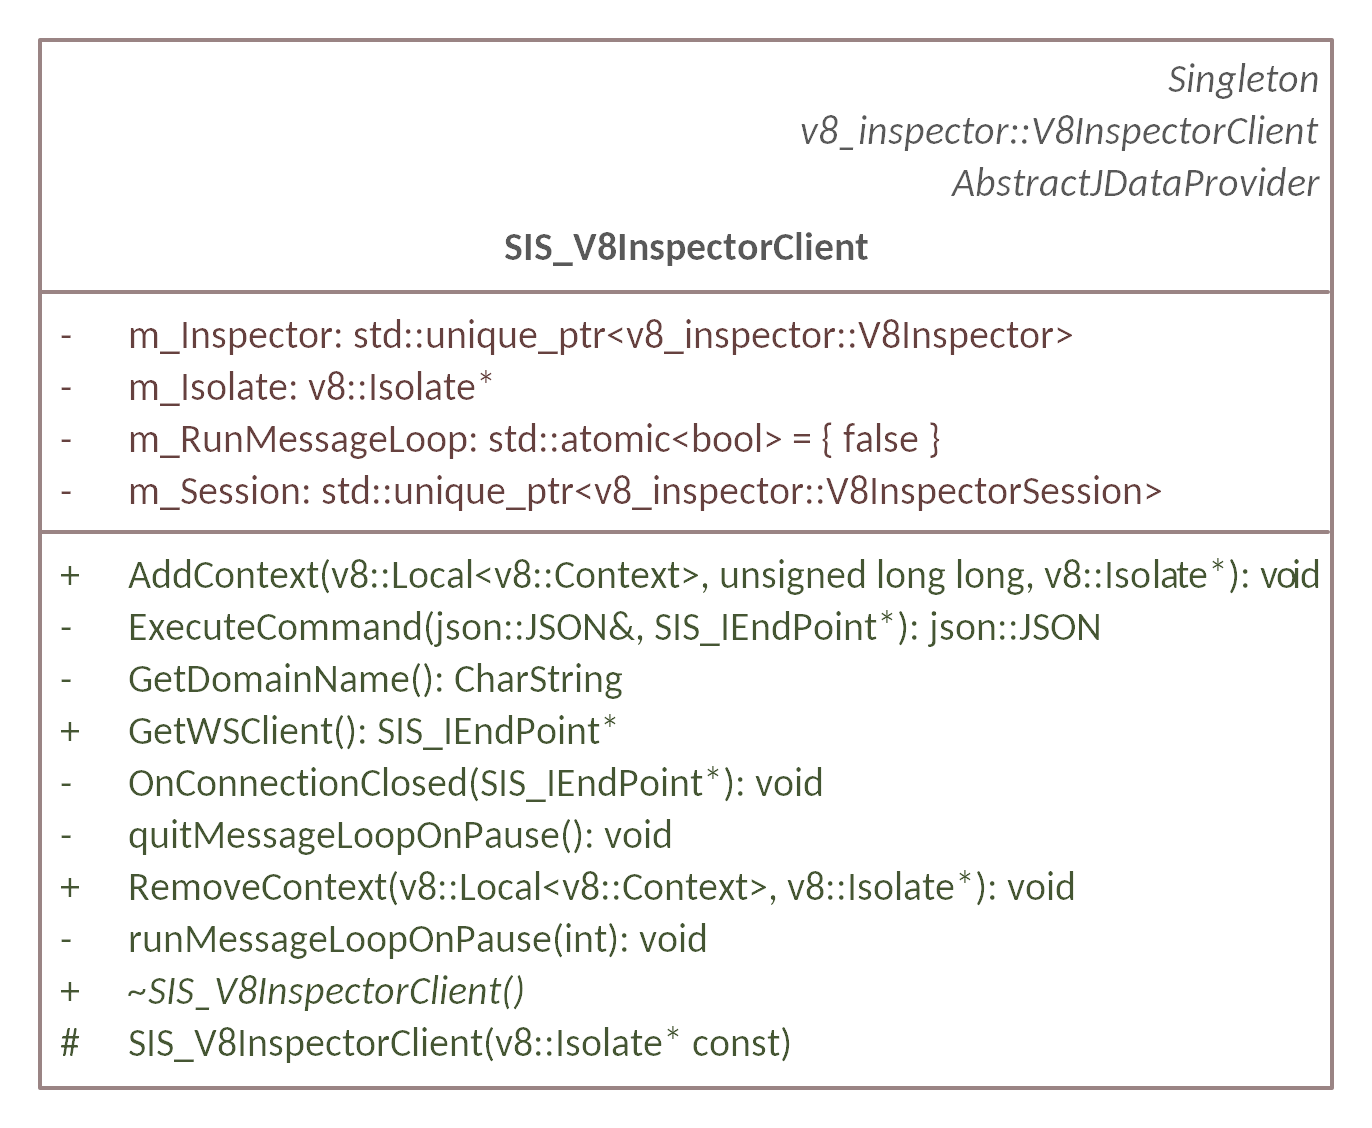
\includegraphics[width=0.63\textwidth]{inspectorclient}
	\caption{Klassendiagramm der imlementierten Programmkomponente.}
	\label{fig:classdiag}
\end{figure}

Die DebugInspector implementiert zusätzlich ein Interface für den in dem \textit{SiPlant} Produkt verwendten Websocket-Server.
Somit können

\subsection{Implementierung der SIS\_InspectorFrontend Klasse}

\begin{figure}[h]
	\centering 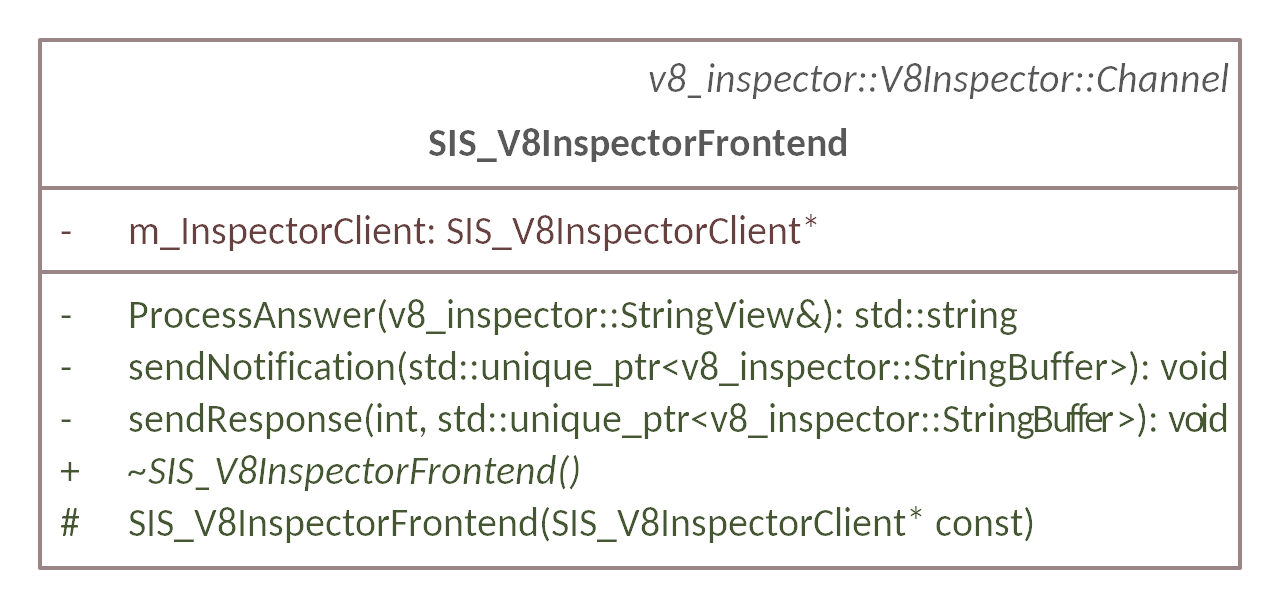
\includegraphics[width=0.63\textwidth]{inspectorfrontend}
	\caption{Klassendiagramm der imlementierten Programmkomponente.}
	\label{fig:classdiag}
\end{figure}

\subsection{Implementierung des ICustomJSCommands Interface}

\begin{figure}[h]
	\centering \includegraphics[width=0.63\textwidth]{icustomjscommands}
	\caption{Klassendiagramm der imlementierten Programmkomponente.}
	\label{fig:classdiag}
\end{figure}

\subsubsection{Konkretisierung DPJSCommands}

\begin{figure}[h]
	\centering 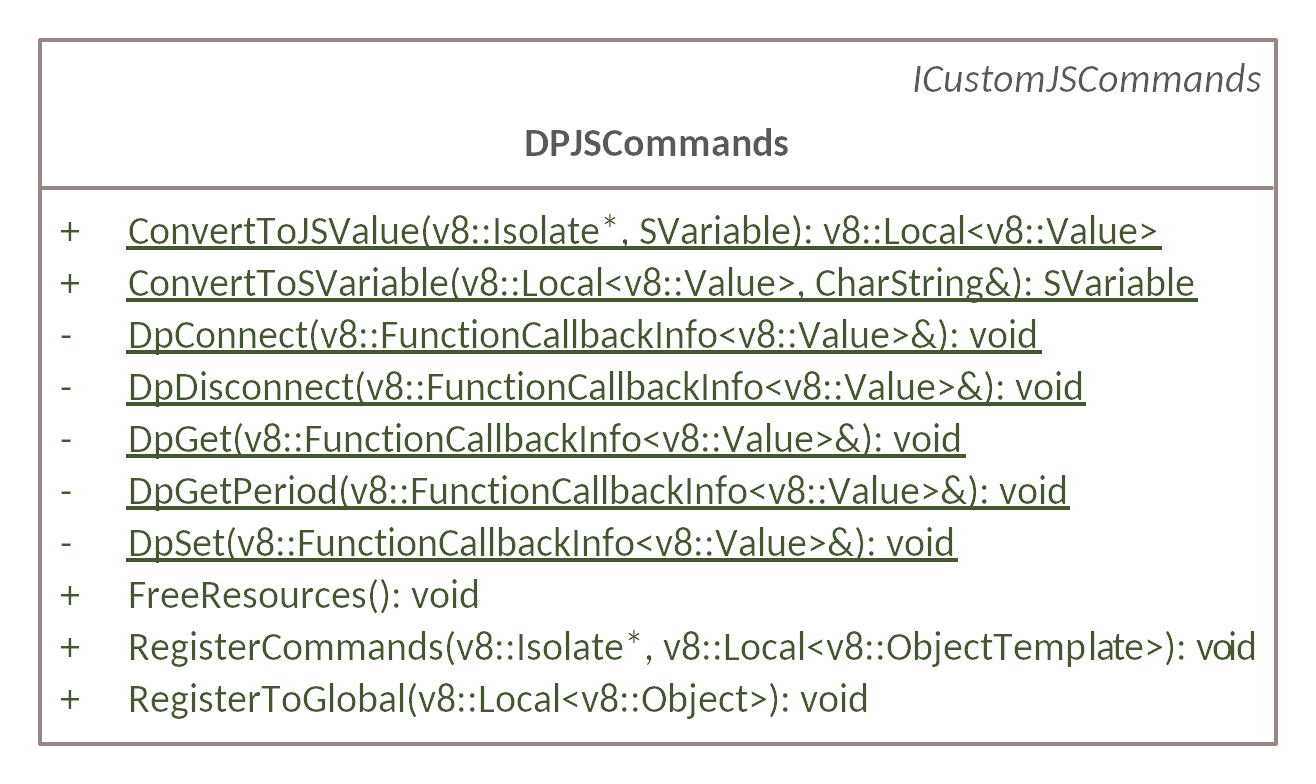
\includegraphics[width=0.63\textwidth]{dpjscommands}
	\caption{Klassendiagramm der imlementierten Programmkomponente.}
	\label{fig:classdiag}
\end{figure}

\subsubsection{Konkretisierung AlertJSCommands}

\begin{figure}[h]
	\centering 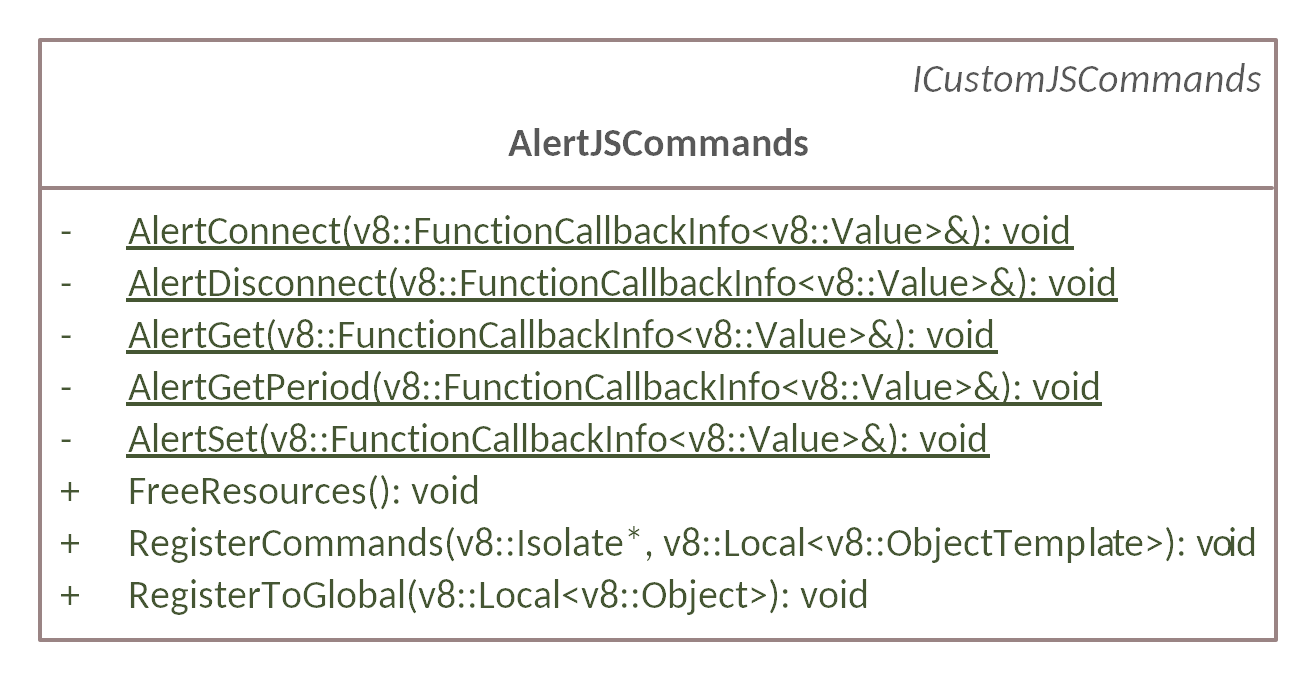
\includegraphics[width=0.63\textwidth]{alertjscommands}
	\caption{Klassendiagramm der imlementierten Programmkomponente.}
	\label{fig:classdiag}
\end{figure}


Dadurch ist es Umsetzungen diese Interfaces können 


\section{Implementierung des Agenten}

Der Agent verwendet die zuvor beschriebene Bibliothek, um Javascript-Dateien ausführen zu können. Die Datei ist über einen Kommandozeilenparameter 
übergebbar. In der Hauptfunktion ist am Anfang das Auslesen des Skriptpfades aus den übergebenen Parametern implementiert. Als Nächstes wird die Verbindung mit dem SCADA-System hergestellt. Darauf folgt das Starten des \textit{SiPlant} Websocket-Servers. Dieser erhält das von der \textit{GetDebuggerInstance()} Funktion zurückgegebenen Observer-Objekt. 
Dadurch ist ein Verbinden mit einer Browser-Entwicklerkonsole möglich. Danach wird vor der Hauptschleife mit dem wiederkehrenden 
\textit{dispatch()} Aufruf das übergebene Skript an die \textit{ExecuteDefault()} Funktion des texit{libV8()}-Singletons weitergereicht. 
Der boolesche Parameter ist hier auf 'false' gesetzt, da der Ausführungskontext nicht zerstört werden soll. Somit ist es möglich, 
eigene Algorithmen zu implementieren und eventorientiert Berechnungen in Javascript durchzuführen.
